% !TeX program = pdflatex
% \documentclass[dvisvgm]{standalone}
\documentclass[tikz,border=5mm]{standalone}
\usepackage{tikz}
\usepackage{pgfplots}
\usetikzlibrary[arrows.meta]
\usetikzlibrary[bending]
\pgfplotsset{compat=1.18}

% Configure for SVG output
% \special{dvisvgm:raw <defs><style type="text/css"><![CDATA[text{font-family:Latin Modern Math}]]></style></defs>}

\begin{document}
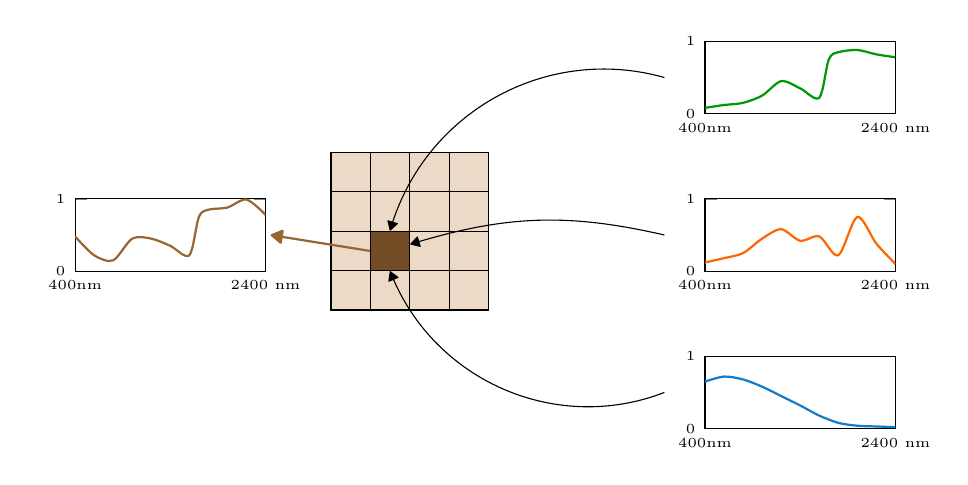
\begin{tikzpicture}
    % 4x4 pixel grid representation
    \foreach \i in {0,1,2,3} {
        \foreach \j in {0,1,2,3} {
            \node[draw, fill=brown!30, minimum size=0.5cm, inner sep=0, anchor=south] at (-0.5+\i*0.5, -0.5+\j*0.5) {};
        }
    }
    % Highlighted target pixel
    \node[draw, fill=brown!60!black, minimum size=0.5cm, inner sep=0, anchor=south] (target-pixel) at (0, 0) {};
    
    \begin{scope}[shift={(-4,0)}]
        \begin{axis}[
            width=4cm, height=2.5cm,
            % xlabel={\footnotesize $\lambda$},
            ylabel={\footnotesize },
            xmin=0, xmax=10,
            ymin=0, ymax=1,
            xtick={0,10},
            xticklabels={\tiny 400nm, \tiny2400 nm},
            ytick={0,  1},
            yticklabels={\tiny 0, \tiny 1},
            grid=major,
            grid style={gray!30}
        ]
    \addplot[brown!80!black, thick, smooth] coordinates {
    (0,0.48) (1,0.22) (2,0.15) (3,0.45) (4,0.45) (5,0.35) 
    (6,0.22) (6.5,0.75) (7,0.85) (8,0.88) (9,0.99) (10,0.78)
    };
    \node at (axis cs:5,1.25)  {\footnotesize \color{brown!80} \textbf{Mixed pixel spectra}};
    \coordinate (spectra-plot) at (axis cs:2,0.5); % Named coordinate
    \end{axis}
    \end{scope}

    % Grass spectrum
    \begin{scope}[shift={(4,2)}]
        \begin{axis}[
            width=4cm, height=2.5cm,
            % % xlabel={\footnotesize $\lambda$},
            ylabel={\footnotesize },
            xmin=0, xmax=10,
            ymin=0, ymax=1,
            xtick={0,10},
            xticklabels={\tiny 400nm, \tiny2400 nm},
            ytick={0,  1},
            yticklabels={\tiny 0, \tiny 1},
            grid=major,
            grid style={gray!30}
        ]
    \addplot[green!60!black, thick, smooth] coordinates {
    (0,0.08) (1,0.12) (2,0.15) (3,0.25) (4,0.45) (5,0.35) 
    (6,0.22) (6.5,0.75) (7,0.85) (8,0.88) (9,0.82) (10,0.78)
    };
    \node at (axis cs:5,1.25) {\footnotesize \color{green!60!black} \textbf{Grass}};
    \coordinate (grass-plot) at (axis cs:2,0.5); % Named coordinate
    \end{axis}
    \end{scope}
    
    % Soil spectrum
    \begin{scope}[shift={(4,0)}]
        \begin{axis}[
            width=4cm, height=2.5cm,
            % xlabel={\footnotesize $\lambda$},
            ylabel={\footnotesize },
            xmin=0, xmax=10,
            ymin=0, ymax=1,
            xtick={0,10},
            xticklabels={\tiny 400nm, \tiny2400 nm},
            ytick={0,  1},
            yticklabels={\tiny 0, \tiny 1},
            grid=major,
            grid style={gray!30}
        ]
    \addplot[orange!80!red, thick, smooth] coordinates {
    (0,0.12) (1,0.18) (2,0.25) (3,0.45) (4,0.58) (5,0.42) 
    (6,0.48) (7,0.22) (8,0.75) (9,0.38) (10,0.10)
    };
    \node at (axis cs:5,1.25) {\footnotesize \color{orange!80!red} \textbf{Soil}};
    \coordinate (soil-plot) at (axis cs:2,0.5); % Named coordinate
    \end{axis}
    \end{scope}
    
    % Water spectrum
    \begin{scope}[shift={(4,-2)}]
        \begin{axis}[
            width=4cm, height=2.5cm,
            % xlabel={\footnotesize $\lambda$},
            ylabel={\footnotesize },
            xmin=0, xmax=10,
            ymin=0, ymax=1,
            xtick={0,10},
            xticklabels={\tiny 400nm, \tiny2400 nm},
            ytick={0,  1},
            yticklabels={\tiny 0, \tiny 1},
            grid=major,
            grid style={gray!30}
        ]
    \addplot[cyan!60!blue, thick, smooth] coordinates {
    (0,0.65) (1,0.72) (2,0.68) (3,0.58) (4,0.45) (5,0.32) 
    (6,0.18) (7,0.08) (8,0.04) (9,0.03) (10,0.02)
    };
    \node at (axis cs:5,1.25) {\footnotesize \color{cyan!60!blue} \textbf{Water}};
    \coordinate (water-plot) at (axis cs:2,0.5); % Named coordinate
    \end{axis}
    \end{scope}
    
    % Arrows pointing to the highlighted pixel
    \draw[-{Triangle[round]}, thin, black] (grass-plot.east) + (-1,0) to[bend right =45] (target-pixel.north) ;%  node[midway, above];% {\small $\mathbf{s}_1$, $a_1 = 0.2$};
    \draw[-{Triangle[round]}, thin, black] (soil-plot.east) + (-1,0) to[bend right =15] (target-pixel) ;%  node[midway, above] {\small $\mathbf{s}_2$, $a_2 = 0.5$};
    \draw[-{Triangle[round]}, thin, black] (water-plot.east) + (-1,0) to[bend left = 45] (target-pixel.south);% node[midway, below];% {\small $\mathbf{s}_3$, $a_3 = 0.3$};
    \draw[{Triangle[round]}-, thick, brown!80!black] (spectra-plot.west) + (2,0) -- (target-pixel.west) ;%  node[midway, below] {};
    
\end{tikzpicture}
\end{document}